\newpage
\section{Recommender Systems}
%---------------------------------------------
\subsection{Recommender ≈ Filtering System}
\begin{itemize}
\item Stable \& long term interest, dynamic info source
\item System must make a delivery decision immediately as a document <<arrives>>
\end{itemize}


\subsubsection{Basic Filtering Question}
Will User U Like Item X?
\begin{itemize}
\item Look at what items U likes, and then check if X is similar 
\begin{itemize}
\item Item similarity $\Rightarrow$ \textbf{content-based filtering}
\end{itemize}

item Look at who likes X, and then check if U is similar 
\begin{itemize}
\item User similarity $\Rightarrow$ \textbf{collaborative filtering}
\end{itemize}
\end{itemize}

%---------------------------------------------
\subsection{Content-Based Filtering}

\subsubsection{A Typical Content-Based Filtering System}
\begin{figure}[H]
    \centering
    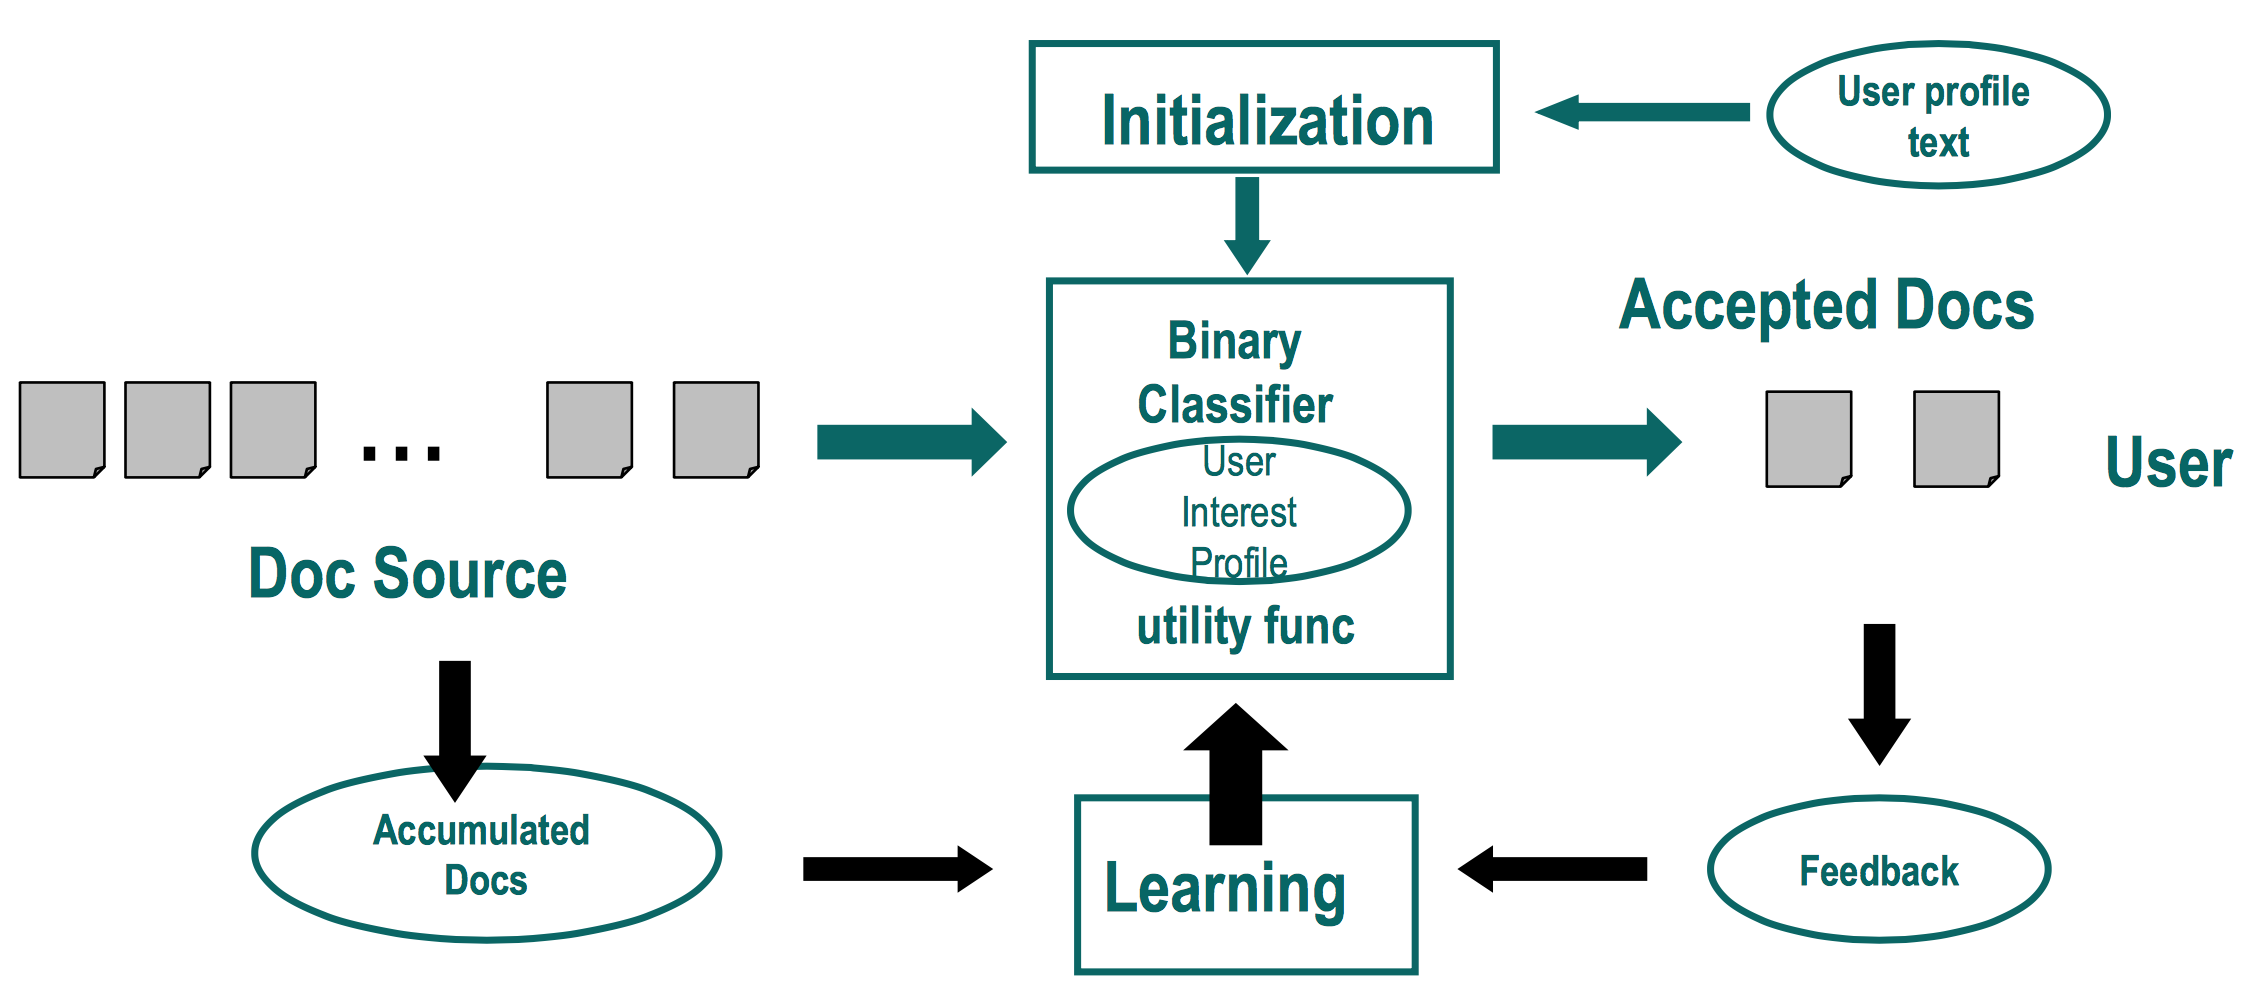
\includegraphics[width=0.9\linewidth]{content_based.png}
\end{figure}

Example of linear utility: 
\begin{equation*}
\text{Linear Utility} = 3 \times \#good - 2 \times \#bad
\end{equation*}


\subsubsection{Three Basic Problems in Content-Based Filtering}
\begin{itemize}
\item Making filtering decision (Binary classifier) 
\begin{itemize}
\item Doc text, profile text $\to$ yes/no
\end{itemize}

\item Initialization
\begin{itemize}
\item Initialize the filter based on only the profile text or very few examples
\end{itemize}

\item Learning from
\begin{itemize}
\item Limited relevance judgments (only on <<yes>> docs) – Accumulated documents
\end{itemize}

\item All trying to maximize the utility
\end{itemize}



\subsubsection{Extend a Retrieval System for Information Filtering}
Content-based recommender system can be built based on a search engine system:
\begin{itemize}
\item <<Reuse>> retrieval techniques to score documents
\item Use a score threshold for filtering decision
\item Learn to improve scoring with traditional feedback
\item New approaches to threshold setting and learning
\end{itemize}


\subsubsection{A General Vector-Space Approach}
\begin{figure}[H]
    \centering
    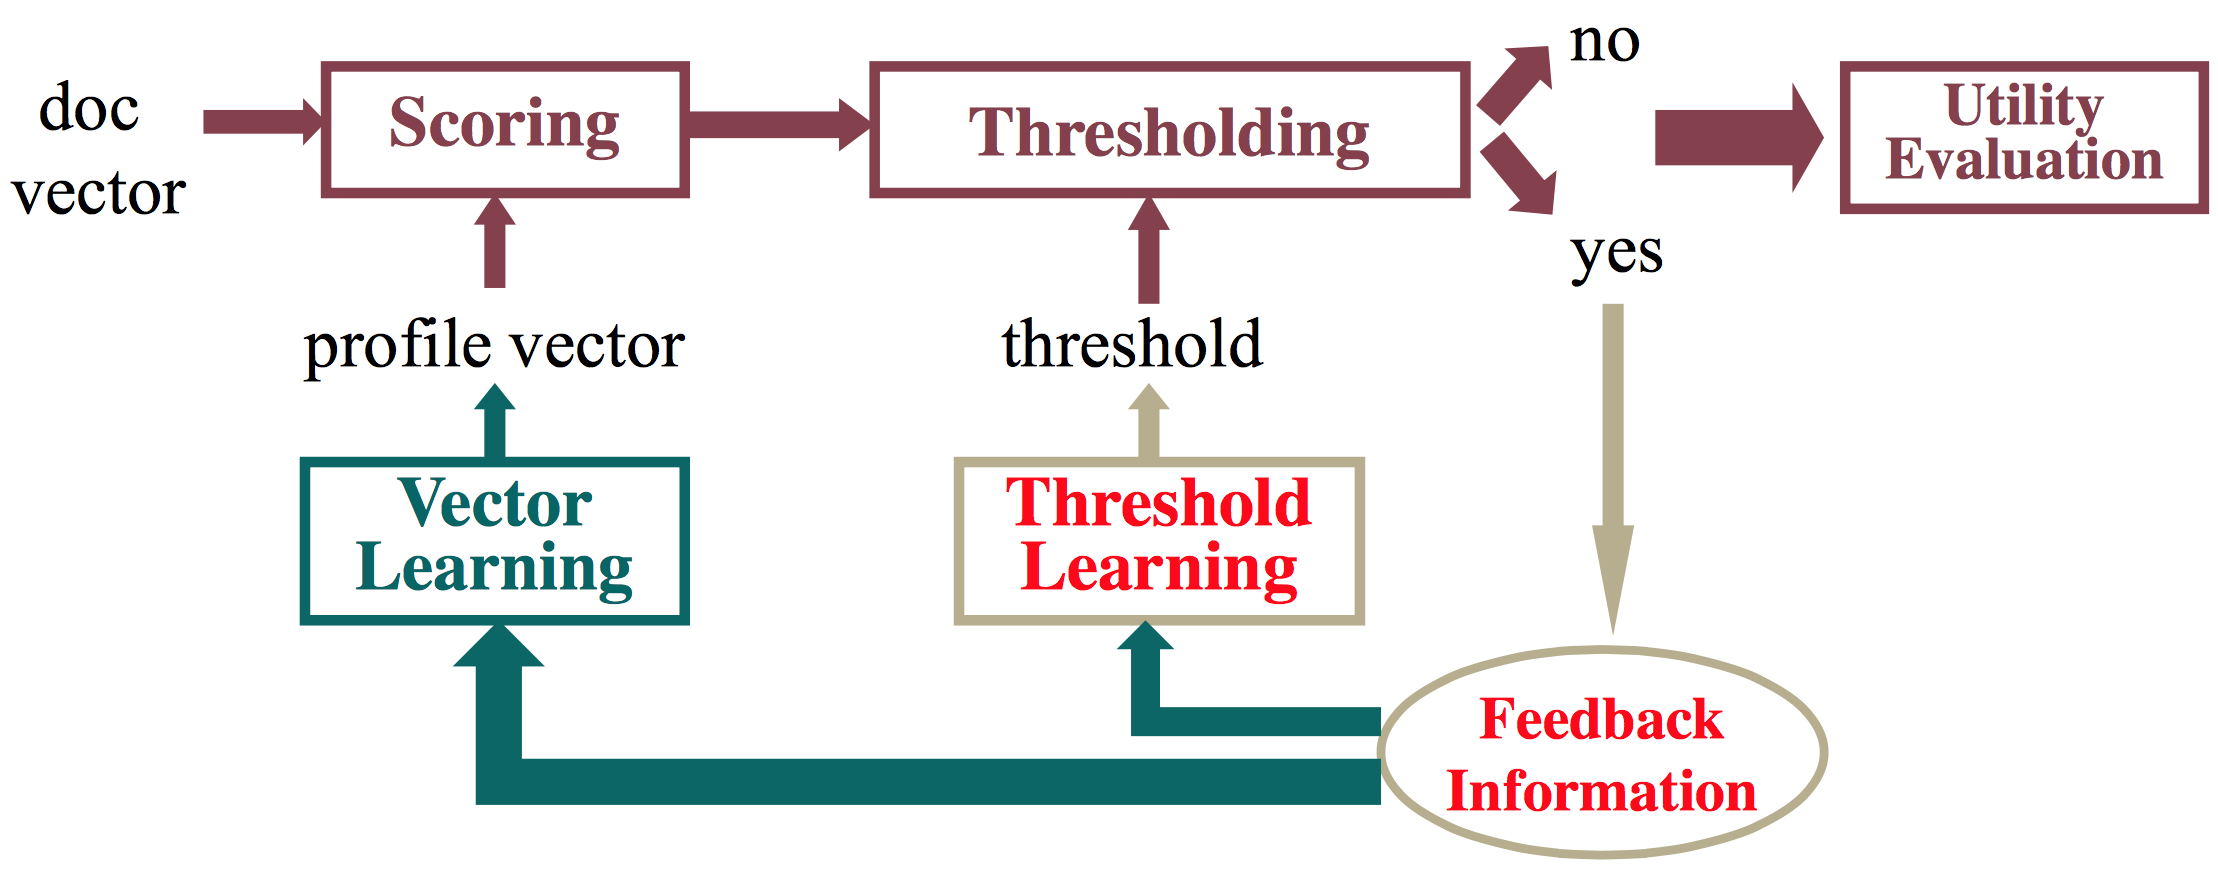
\includegraphics[width=0.9\linewidth]{content_based_vsm.png}
\end{figure}


\subsubsection{Difficulties in Threshold Learning}
\begin{itemize}
\item Censored data (judgments only available on delivered documents)
\item Little or none labeled data
\item Exploration vs. Exploitation
\end{itemize}


\subsubsection{Empirical Utility Optimization}
\begin{itemize}
\item Basic idea
\begin{itemize}
\item Compute the utility on the training data for each candidate score
threshold
\item Choose the threshold that gives the maximum utility on the training data set
\end{itemize}

\item Difficulty: Biased training sample!
\begin{itemize}
\item We can only get an upper bound for the true optimal threshold 
\item Could a discarded item be possibly interesting to the user?
\end{itemize}

\item Solution:
\begin{itemize}
\item Heuristic adjustment (lowering) of threshold
\end{itemize}
\end{itemize}


\subsubsection{Beta-Gamma Threshold Learning}

\begin{figure}[H]
    \centering
    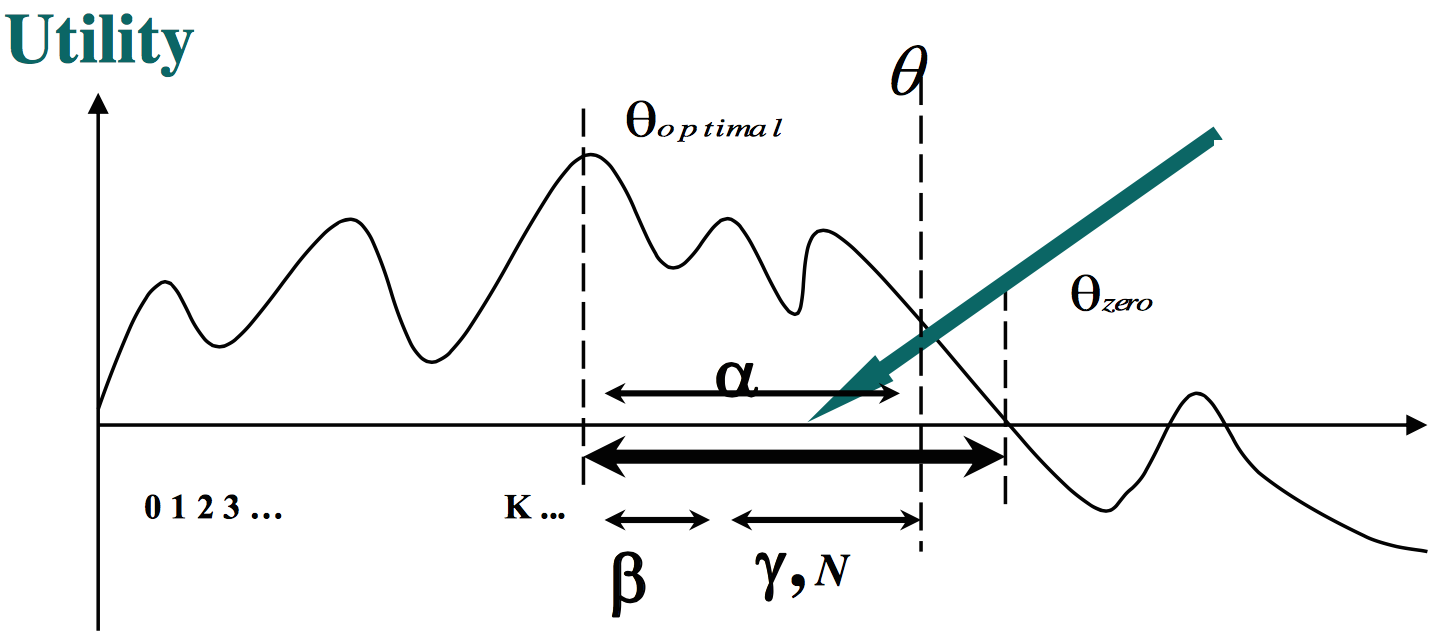
\includegraphics[width=0.7\linewidth]{beta_gamma.png}
\end{figure}

Encourage exploration of threshold up to $\theta_{zero}$:
\begin{equation*}
\theta = \alpha \times \theta_{zero} + (1-\alpha) \times \theta_{optimal}
\end{equation*}

The more examples, the less exploration (closer to $\theta_{optimal}$):
\begin{equation*}
\alpha = \beta + (1-\beta) \times e^{-N\gamma}, \text{ where }\beta,\gamma \in [0, 1]
\end{equation*}

\begin{itemize}
\item Pros:
\begin{itemize}
\item Explicitly addresses exploration-exploitation tradeoff (<<Safe>>
exploration)
\item Arbitrary utility (with appropriate lower bound)
\item Empirically effective
\end{itemize}

\item Cons:
\begin{itemize}
\item Purely heuristic
\item Zero utility lower bound often too conservative
\end{itemize}
\end{itemize}



%---------------------------------------------
\subsection{Collaborative Filtering}

\subsubsection{What is Collaborative Filtering (CF)?}
\begin{itemize}
\item Making filtering decisions for an individual user based on the judgments of other users
\item Inferring individual’s interest/preferences from that of other similar users
\item User similarity can be judged based on their similarity in preferences on a common set of items
\end{itemize}

CF assumptions
\begin{itemize}
\item Users with the same interest will have similar preferences
\item Users with similar preferences probably share the same interest
\item Sufficiently large number of user preferences are available (if not, there will be a <<cold start>> problem)
\end{itemize}


\newpage
\subsubsection{Memory-based Approaches to Collaboration Filtering Problem}

\begin{multicols}{2}

\begin{figure}[H]
    \centering
    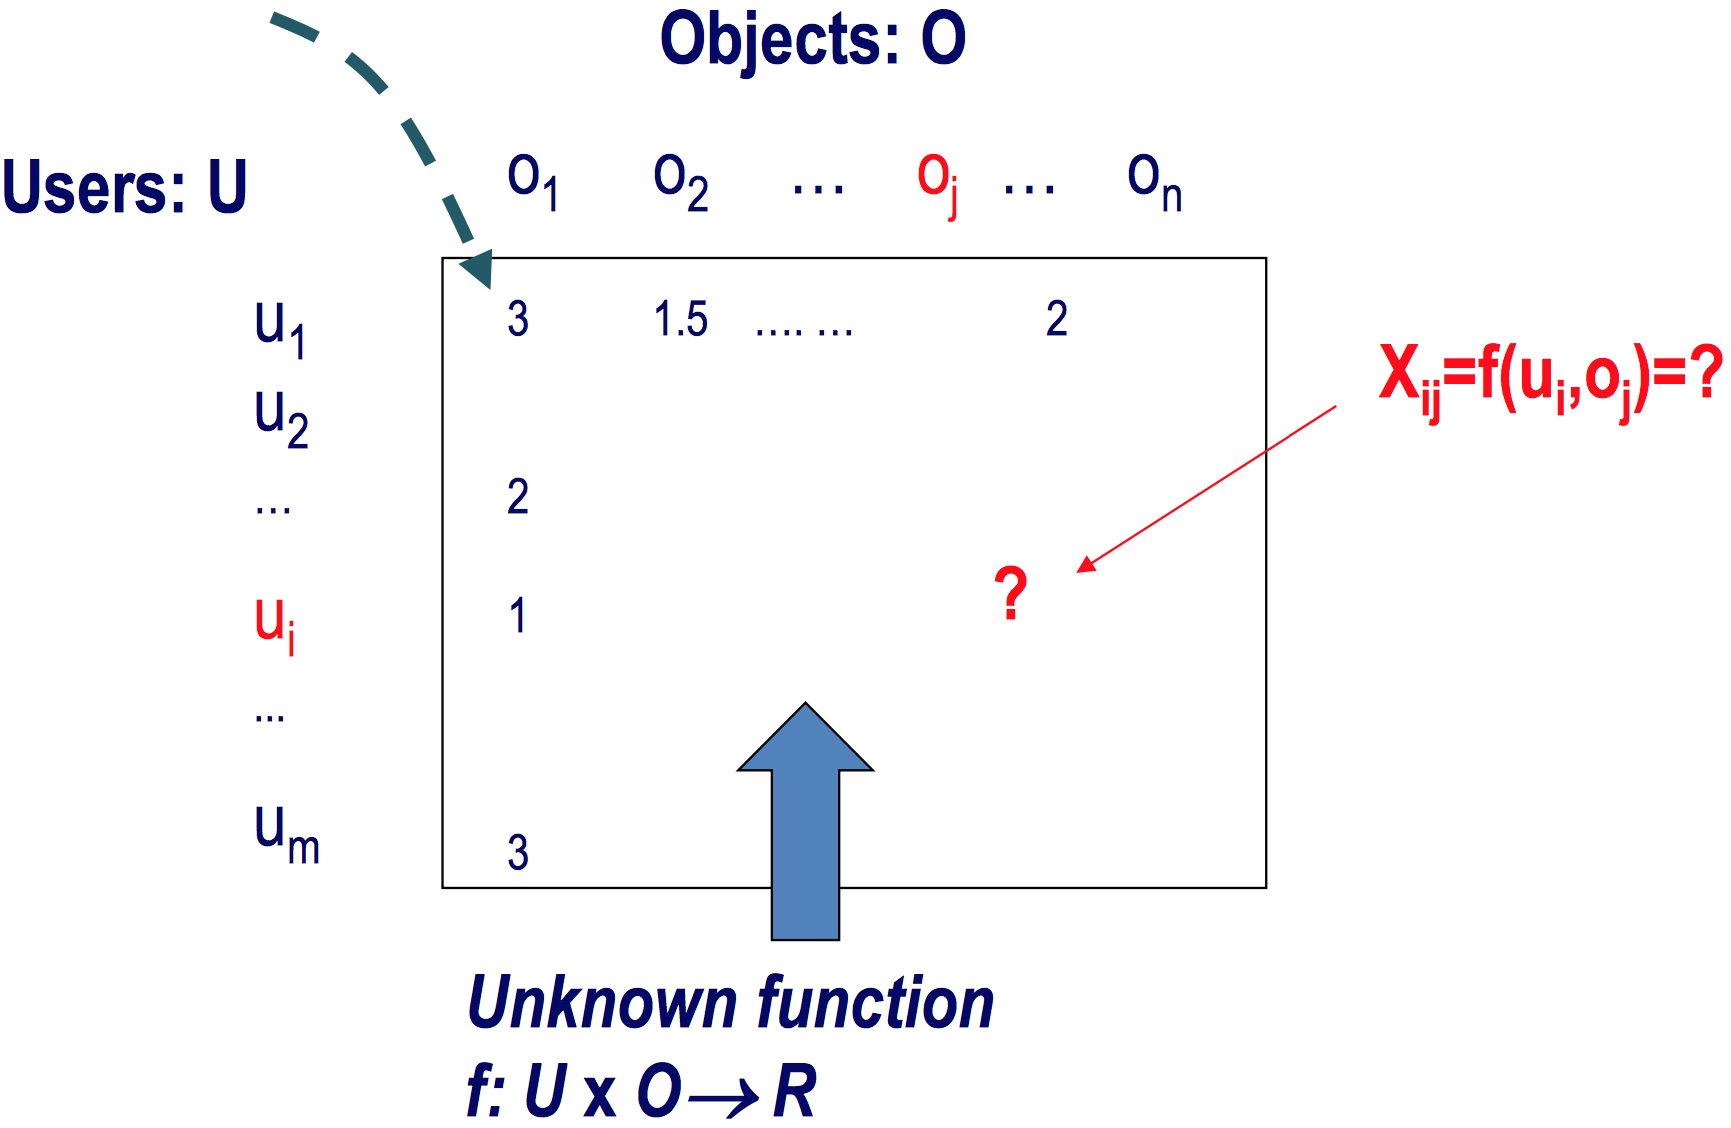
\includegraphics[width=\linewidth]{collaborative_problem.png}
\end{figure}

\columnbreak

\begin{itemize}
\item Assume we have $m$ users ($u_i$) and $n$ objects $o_j$
\item $x_{ij}$: rating of object $o_j$ by user $u_i$
\item $n_i$: average rating of all objects by user $u_i$ 
\item Normalized ratings: $v_{ij} = x_{ij} - n_i$
\end{itemize}
\end{multicols}

Prediction of rating of object $o_j$ by user $u_a$:
\begin{equation*}
\hat{v_{aj}} = \frac{\sum\limits_{i=1}^m v_{a,i} v_{ij}}{\sum\limits_{i=1}^m v_{a,i}}, \;\hat{x_{aj}} = \hat{v_{aj}} + n_a
\end{equation*}



\subsubsection{User Similarity Measures}
\begin{itemize}
\item Pearson correlation
\begin{equation*}
w_p(a, j) = \frac{\sum_j (x_{aj} - n_a)(x_{ij} - n_i)}{\sqrt{\sum_j (x_{aj} - n_a)^2 \sum_j(x_{ij} - n_i)^2}}
\end{equation*}

\item Cosine measure
\begin{equation*}
w_c(a, j) = \frac{\sum_j x_{aj} x_{ij}}{\sqrt{\sum_j x_{aj}^2 \sum_j x_{ij}^2}}
\end{equation*}
\end{itemize}


\subsubsection{Improving User Similarity Measures}
\begin{itemize}
\item Dealing with missing values: set to default ratings
\begin{itemize}
\item average ratings
\item iterate unknown ratings calculations followed by similarity measure calculation
\end{itemize}

\item Inverse User Frequency (IUF): similar to IDF
\end{itemize}



\subsubsection{Summary}
\begin{itemize}
\item Filtering/Recommendation is <<easy>>
\begin{itemize}
\item The user’s expectation is low
\item Any recommendation is better than none
\end{itemize}

\item Filtering is <<hard>>
\begin{itemize}
\item Must make a binary decision, though ranking is also possible
\item Data sparseness (limited feedback information)
\item <<Cold start>> (little information about users at the beginning)
\end{itemize}
\end{itemize}



\subsubsection{Recommended reading}
\begin{itemize}
\item Francesco Ricci, Lior Rokach, Bracha Shapira, Paul B. Kantor. \href{http://www.cs.bme.hu/nagyadat/Recommender_systems_handbook.pdf}{<<Recommender Systems Handbook>>}. Springer 2011.
\end{itemize}
